%=====================================================================
% Workshop 5 — Generative Adversarial Networks on MovieLens 32M
% Team 7 — Universidad Distrital Francisco Jose de Caldas
%
% Compile on Overleaf with pdfLaTeX. Figures go in docs/w5/figures/.
% This file follows the two-column, numbered-section style of the
% Workshop 2 and Workshop 4 reports of the same team.
%=====================================================================
\documentclass[10pt,twocolumn]{article}

\usepackage[utf8]{inputenc}
\usepackage[T1]{fontenc}
\usepackage{amsmath,amssymb}
\usepackage{graphicx}
\usepackage{booktabs}
\usepackage{geometry}
\usepackage{caption}
\usepackage{hyperref}
\usepackage{xcolor}
\usepackage{float}

\geometry{margin=1.9cm}
\captionsetup{font=small}
\setlength{\parskip}{2pt}

\title{\vspace{-1.0cm}\textbf{\Large Synthetic Interaction Generation on the MovieLens 32M
Dataset with Vanilla GANs, WGAN-GP, and Conditional GANs}}

\author{
Andr\'es Felipe Ruiz Vasallo\textsuperscript{1}, \;
Josep Emanuel Le\'on Joya\textsuperscript{1}, \;
Matthew Stev Toro Mondrag\'on\textsuperscript{1} \\[2pt]
\small \textsuperscript{1}Team 7 --- Computer Engineering Program, Universidad Distrital Francisco Jos\'e de Caldas \\
\small \texttt{\{afruizv, jeleonj, mstorom\}@udistrital.edu.co} \\
\small GitHub Repository: \url{https://github.com/AndresRuiz14502/Machine_Learning.git} \\[2pt]
\small Workshop No.\ 5 --- Generative Adversarial Networks
}
\date{}

\begin{document}
\maketitle

%=====================================================================
\begin{abstract}
\small
\textbf{Abstract}---Supervised, reinforcement, and unsupervised models learn how to score
or organize user--movie interactions, but they do not learn how to \emph{generate} new
interactions. In this work we study Generative Adversarial Networks (GANs) as a way to
produce synthetic interaction profiles for the MovieLens 32M (\texttt{ml-32m}) dataset, and
we test whether this synthetic data can help a downstream task through data augmentation.
Building on our Workshops 1, 2, and 4 studies, we reuse the same leak-free chronological
split (1{,}895{,}184 training, 33{,}092 validation, and 23{,}551 test interactions across
14{,}998 users and 11{,}589 movies) and the same 64-dimensional interaction profiles from
Workshop 4. We train a Vanilla GAN with binary cross-entropy and one-sided label smoothing,
a Wasserstein GAN with gradient penalty (WGAN-GP), and an optional conditional GAN (cGAN)
on the binary \texttt{like} label. Because our data is tabular and not images, we evaluate
generation quality with domain-specific metrics instead of the Inception Score. The WGAN-GP
clearly produces better samples than the Vanilla GAN, reaching a tabular Fr\'echet distance
of 0.1107 versus 0.7327 and a lower correlation error (0.0228 versus 0.0542), while neither
model shows mode collapse (diversity ratio 0.9687 and 0.9379). In the data augmentation
experiment, adding synthetic data to a downstream \texttt{like} classifier changes the test
F1 only marginally (baseline F1 = 0.6650; best case +0.0028 with WGAN-GP), which we interpret
as a consequence of already having abundant real data. This means that GAN-based augmentation
does not hurt the model but also does not help much in this regime, a result that is coherent
with the data augmentation literature.

\vspace{4pt}
\noindent\textbf{Index Terms}---Generative adversarial networks, WGAN-GP, conditional GAN,
synthetic data, data augmentation, MovieLens 32M, tabular generation.
\end{abstract}

%=====================================================================
\section{Motivation: Generative Modeling in Recommendation}

\subsection{Why Generate Synthetic Interactions for MovieLens 32M?}

In our previous workshops we studied the MovieLens 32M dataset from three different angles.
In Workshops 1 and 2 we used supervised learning to predict ratings and the binary
\texttt{like} label~\cite{koren2009,he2017}. In Workshop 3 we used reinforcement learning to
recommend movies as a sequential decision process. In Workshop 4 we used unsupervised
autoencoders and $\beta$-VAEs to compress and organize the interactions without labels.
All of these models \emph{read} the data and learn a function over it. However, none of them
learns to \emph{create} new data. This is the gap that generative models fill.

A Generative Adversarial Network (GAN)~\cite{goodfellow2014} trains two networks against each
other. A generator $G$ maps a noise vector $z$ to a synthetic sample, and a discriminator $D$
tries to tell real samples from fake ones. At the end of training, $G$ should produce samples
that look like the real data. This means that the model learns the distribution of the
interactions, not only a decision boundary. Generative models are useful for two practical
reasons that matter in recommendation. First, they can produce synthetic data to augment a
small or unbalanced training set~\cite{fridadar2018}. Second, they are a good way to study the
structure of the data, because a generator that produces realistic samples has implicitly
captured the correlations between the features.

In this work we focus on the central questions of the workshop: can we build a GAN that
generates realistic synthetic data from our domain, and can that synthetic data improve our
overall system through augmentation? We answer both questions using the same data and the
same splits as the previous workshops, so the comparison is fair.

\subsection{Tabular Generation over 64-Dimensional Profiles}

An important design decision is \emph{what} the GAN should generate. The MovieLens ratings are
not images, so the image-oriented GAN recipes (convolutions, transposed convolutions) do not
apply directly. Instead, we reuse the 64-dimensional leak-free interaction profiles that we
built in Workshop 4. Each profile $x_{ui}\in\mathbb{R}^{64}$ describes one user--movie
interaction and combines historical user/item statistics, multi-hot genres and temporal
features, frozen collaborative (GMF) interactions from Workshop 2, and normal-manifold
compatibility deviations. Because these vectors are tabular and continuous, we build the
generator and the discriminator with fully-connected layers, as the workshop guidelines
recommend for tabular data. This reuse also keeps the experiment leak-free by construction,
because the 64-D vectors were already fitted strictly on the training split.

%=====================================================================
\section{Background and Related Work}

\subsection{Vanilla GAN and the Minimax Objective}

The original GAN~\cite{goodfellow2014} defines a two-player minimax game between the generator
$G$ and the discriminator $D$:
\begin{equation}
\min_{G}\max_{D}\; V(D,G) =
\mathbb{E}_{x\sim p_{\text{data}}}[\log D(x)] +
\mathbb{E}_{z\sim p_z}[\log(1 - D(G(z)))].
\label{eq:gan}
\end{equation}
Here $D(x)$ is the probability that $x$ is real. The discriminator wants to maximize this
value, and the generator wants to minimize it, so that $D$ can no longer separate real from
fake. In practice we train $D$ on a batch of real and fake samples, and then train $G$ so that
$D$ classifies its output as real. The DCGAN paper~\cite{radford2015} later gave useful
architectural rules (batch normalization, ReLU in the generator, LeakyReLU in the
discriminator), which we follow in our fully-connected version.

\subsection{Wasserstein GAN with Gradient Penalty}

A well-known problem of the Vanilla GAN is unstable training: the discriminator can become too
strong, the gradient for the generator vanishes, and the loss curves do not say much about the
real quality. The Wasserstein GAN~\cite{arjovsky2017} replaces the classification objective by
the Wasserstein distance, which gives a smoother and more meaningful signal. Instead of a
discriminator with a sigmoid output, it uses a \emph{critic} that outputs a real-valued score.
To enforce the required Lipschitz constraint, Gulrajani et al.~\cite{gulrajani2017} proposed
the gradient penalty (WGAN-GP), which penalizes the norm of the critic gradient on points
interpolated between real and fake samples:
\begin{equation}
\text{GP} = \lambda\,
\mathbb{E}_{\hat{x}}\big[(\lVert \nabla_{\hat{x}} D(\hat{x}) \rVert_2 - 1)^2\big],
\quad \hat{x} = \epsilon x + (1-\epsilon)\tilde{x},
\label{eq:gp}
\end{equation}
with $\epsilon\sim U[0,1]$ and $\lambda=10$. The critic is trained several steps per generator
step. For this reason WGAN-GP is today a standard and more stable way to train GANs, and we use
it as the stable alternative to the Vanilla GAN.

\subsection{Conditional GAN}

A conditional GAN (cGAN) lets us control the class of the generated sample by giving the label
to both $G$ and $D$~\cite{isola2016}. In our domain the discrete label is $\texttt{like}\in
\{0,1\}$ (the user liked the movie or not). This is useful because the unconditional GANs learn
mostly the majority class; with a cGAN we can also generate the minority class and build a more
balanced synthetic set for augmentation.

\subsection{Generation Quality Metrics for Tabular Data}

The Inception Score~\cite{salimans2016} and the Fr\'echet Inception Distance~\cite{heusel2017}
were designed for images, because they use a pretrained Inception network. Our data is tabular,
so these scores do not apply directly. For this reason we use domain-specific metrics, as the
workshop allows. We compute a tabular Fr\'echet distance directly on the 64-D feature space, we
measure how well the generator preserves the correlation structure of the features, and we
measure the diversity of the generated samples to detect mode collapse. We also do a visual
inspection of real versus generated samples.

\subsection{GANs for Data Augmentation}

Frid-Adar et al.~\cite{fridadar2018} showed a clear augmentation pipeline: train a GAN, generate
synthetic data, add it to the training set, and measure if a downstream classifier improves.
We follow the same idea, but we must adapt the downstream model to our setting, as we explain
in the methodology.

%=====================================================================
\section{Methodology}

\subsection{Dataset and Leak-Free Split}

We use the MovieLens 32M dataset~\cite{harper2015} and we keep exactly the same preprocessing
and chronological split as Workshops 1, 2, and 4, so the results are comparable. Using a fixed
seed (\texttt{seed}~$=42$), we sample 15{,}000 complete users and apply iterative 10-core
filtering, which gives 2{,}368{,}980 ratings across 14{,}998 users and 11{,}589 movies. All
interactions are sorted by timestamp and split globally into 80\% training, 10\% validation,
and 10\% test. After removing cold-start rows (users or movies not seen in training), the final
sizes are 1{,}895{,}184 training, 33{,}092 validation, and 23{,}551 test interactions. This is
the same split reported in our previous workshops.

\subsection{64-Dimensional Interaction Profiles}

Instead of generating raw ratings, the GAN works on the 64-dimensional leak-free interaction
profiles that we built in Workshop 4. Each interaction $(u,i)$ is a continuous vector
$x_{ui}\in\mathbb{R}^{64}$ that joins four groups of features: historical user/item statistics,
multi-hot genres and temporal features, frozen collaborative (GMF) interactions from Workshop 2,
and normal-manifold compatibility deviations. These vectors are produced by the same Workshop 4
function, so all the statistics used to build them come only from the training split. This means
the representation is leak-free by construction, and the GAN cannot see information from the
validation or test periods.

The generator uses a $\tanh$ output, which produces values in $[-1,1]$, but the Workshop 4
vectors live in a wider range. For this reason we rescale the data to $[-1,1]$ with a min--max
transform whose minimum and range are computed \emph{only} on the training profiles. We store
these limits so that we can map the synthetic samples back to the original scale when we need
them for the downstream task. Fixing the scaling on training data is another point where we
avoid leakage.

\subsection{Generator, Discriminator, and Critic}

All models share the same generator $G$. It is a fully-connected network that maps a noise
vector $z\in\mathbb{R}^{64}$, $z\sim\mathcal{N}(0,I)$, to a synthetic profile
$\hat{x}\in\mathbb{R}^{64}$:
\begin{equation}
G:\; z \;\rightarrow\; 256 \;\rightarrow\; 256 \;\rightarrow\; 64,
\label{eq:gen}
\end{equation}
with batch normalization and ReLU in the hidden layers and a $\tanh$ output, following the DCGAN
guidelines adapted to tabular data. For the Vanilla GAN, the discriminator $D$ is also
fully-connected ($64\rightarrow256\rightarrow256\rightarrow1$) with LeakyReLU, dropout, and a
sigmoid output, so $D(x)\in[0,1]$ is the probability of being real. For the WGAN-GP, the critic
$C$ has the same shape but \emph{without} the sigmoid, so it outputs a real-valued score. We also
replace batch normalization by layer normalization in the critic, because batch normalization
mixes samples inside the batch and this breaks the per-sample gradient penalty of
Equation~\eqref{eq:gp}.

For the conditional GAN, both the generator and the discriminator receive the class label
through a small embedding that is concatenated to their input. In this way we can ask the
generator for samples of a chosen class, $G(z,y)$ with $y\in\{0,1\}$.

\subsection{Training Protocol}

We train every model for 120 epochs (that is, more than the 100 epochs required), with a batch
size of 256 and Adam optimizers with learning rate $2\times10^{-4}$ and $\beta=(0.5,0.9)$.

\paragraph{Vanilla GAN.} We use the binary cross-entropy loss. For each batch we first train
$D$ on real and fake samples, and then we train $G$ so that $D$ labels its output as real. We
apply one-sided label smoothing, using $0.9$ instead of $1.0$ for the real labels, which is a
standard trick to stop the discriminator from becoming too confident. We log the discriminator
accuracy on real and fake batches and the generator loss per epoch, and we save generated
samples every 10 epochs.

\paragraph{WGAN-GP.} We use the same generator and the critic described above. The critic loss
is the Wasserstein term plus the gradient penalty of Equation~\eqref{eq:gp} with $\lambda=10$.
We train the critic 5 steps for every 1 generator step, as in the original WGAN-GP schedule. We
log the critic loss and the Wasserstein distance per epoch, which should decrease and then stay
stable if the training is healthy.

\paragraph{Conditional GAN.} The cGAN is trained like the Vanilla GAN (binary cross-entropy,
label smoothing), but $G$ and $D$ are conditioned on the \texttt{like} label. Because Workshop 4
only exposes both classes in the validation split, we train the cGAN on the validation profiles,
which are held-out and contain both \texttt{like}~$=1$ and \texttt{like}~$=0$. This keeps the
test split unseen.

\subsection{Downstream Model for the Augmentation Experiment}

The augmentation experiment needs a downstream model. The natural choice would be the Workshop 2
model (\texttt{HybridNeuMF}), but that model takes user and item \emph{indices} as input and
learns its own embeddings; it does not take feature vectors. A GAN that generates 64-D vectors
does not produce valid user/item indices, so we cannot retrain \texttt{HybridNeuMF} on synthetic
vectors without inventing an index assignment. For this reason we use a small tabular classifier
that predicts the \texttt{like} label directly from the 64-D vector. This is exactly the
Frid-Adar pipeline~\cite{fridadar2018}: train a GAN, generate synthetic data, add it to the
downstream training set, and measure the change. The classifier is a small multi-layer
perceptron ($64\rightarrow64\rightarrow1$) trained with a fixed budget (40 epochs, Adam,
$10^{-3}$) so that every condition has the same training effort and the comparison is fair.

We compare four conditions, all evaluated on the same held-out test split:
\begin{itemize}
\item \textbf{(a) Real only}: the baseline classifier trained on real data.
\item \textbf{(b) Real + Vanilla}: real data plus synthetic samples from the Vanilla GAN.
\item \textbf{(c) Real + WGAN-GP}: real data plus synthetic samples from the WGAN-GP.
\item \textbf{(d) Real + cGAN}: real data plus balanced synthetic samples from the cGAN.
\end{itemize}
Conditions (b) and (c) are the ones required by the workshop. We add condition (d) because the
unconditional GANs learn mostly the majority class (\texttt{like}~$=1$), so they add data that
is already well represented. The cGAN can generate the minority class (\texttt{like}~$=0$), so
condition (d) tests whether a more balanced synthetic set changes the result. The downstream
classifier is trained on the validation split (which has both classes) and evaluated on the test
split, both from the same leak-free split as the previous workshops.

\subsection{Generation Quality Evaluation}

To evaluate the samples we generate between 1{,}000 and 5{,}000 synthetic profiles and compare
them with the real training profiles. We report four domain-specific metrics. The tabular
Fr\'echet distance measures the distance between the mean and covariance of the real and the
generated profiles,
\begin{equation}
\text{FD} = \lVert \mu_r - \mu_g \rVert_2^2 +
\mathrm{Tr}\!\left(\Sigma_r + \Sigma_g - 2(\Sigma_r\Sigma_g)^{1/2}\right),
\label{eq:fd}
\end{equation}
where a lower value is better. The correlation error is the mean absolute difference between the
feature correlation matrices of the real and the generated data. We also report the mean
absolute error of the per-feature means and standard deviations. Finally, the diversity ratio is
the mean pairwise distance of the generated samples divided by the same quantity on the real
samples; a value close to $1$ means good coverage, and a small value is a sign of mode collapse.

%=====================================================================
\section{Results}

\subsection{Training Dynamics and Stability}

Figure~\ref{fig:curves} shows the training curves of the two unconditional models. The Vanilla
GAN is stable: the discriminator loss stays around $1.3$ and the generator loss grows slowly
from $0.86$ to $1.11$ over the 120 epochs, without any collapse. The discriminator accuracy on
real samples stays low (around $0.36$--$0.50$) and the accuracy on fake samples stays around
$0.83$. This means that the discriminator never becomes perfect, so the generator always has a
useful gradient to learn from. This is the healthy regime that one-sided label smoothing is
meant to produce.

The WGAN-GP shows an even clearer picture. The Wasserstein distance drops quickly from $1.99$
to about $0.41$ and then stays stable for the rest of the training. This is exactly the
behavior that WGAN-GP is expected to show: a loss curve that decreases and then stabilizes,
which is easier to read than the Vanilla GAN losses. The generator loss keeps growing in
absolute value (down to $-13.9$), but this is normal in WGAN-GP and its magnitude does not
indicate quality by itself, so we do not read it as a problem.

\begin{figure}[t]
\centering
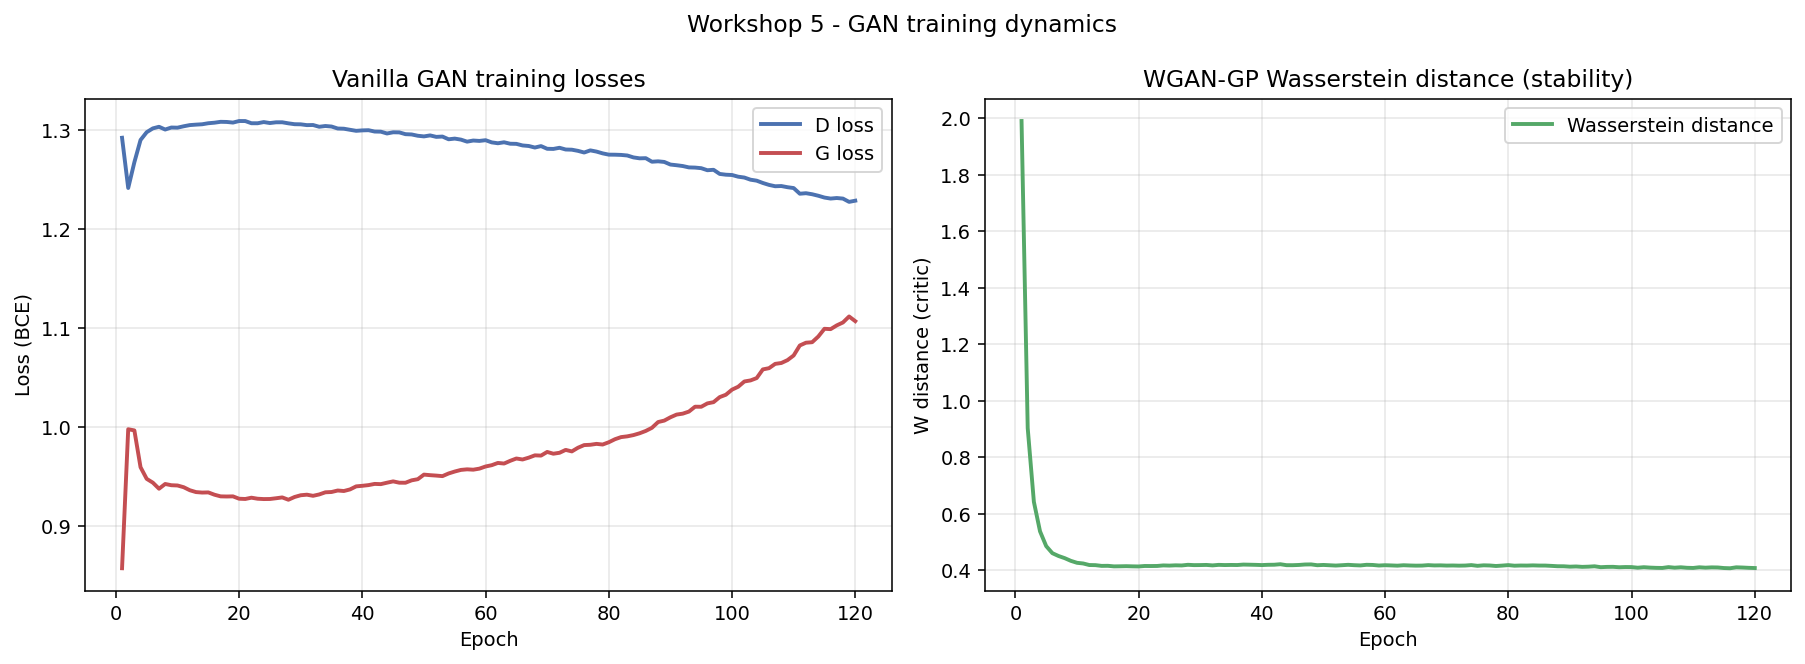
\includegraphics[width=\columnwidth]{figures/training_curves.png}
\caption{Training dynamics over 120 epochs. Left: Vanilla GAN discriminator and generator
losses (BCE). Right: WGAN-GP Wasserstein distance, which decreases from 1.99 and then stays
stable around 0.41. Source: \texttt{runs/workshop5/training\_curves.png}.}
\label{fig:curves}
\end{figure}

\subsection{Generation Quality: Vanilla GAN vs. WGAN-GP}

Table~\ref{tab:quality} reports the domain-specific quality metrics on 5{,}000 generated
samples. The WGAN-GP is better in every metric. Its tabular Fr\'echet distance is $0.1107$,
which is about $6.6$ times lower than the $0.7327$ of the Vanilla GAN. It also matches the
feature correlations better ($0.0228$ versus $0.0542$) and the per-feature means and standard
deviations better. This means that the WGAN-GP captures the structure of the real profiles more
faithfully. Importantly, neither model shows mode collapse: the diversity ratio is $0.9687$ for
WGAN-GP and $0.9379$ for the Vanilla GAN, both close to $1$, so the generated samples cover
almost the same spread as the real ones.

\begin{table}[t]
\centering
\caption{Generation quality on 5{,}000 synthetic samples (domain-specific metrics). Lower is
better except the diversity ratio, where a value close to 1 is best. Source:
\texttt{runs/workshop5/gan\_quality\_metrics.json}.}
\label{tab:quality}
\small
\begin{tabular}{lcc}
\toprule
Metric & Vanilla GAN & WGAN-GP \\
\midrule
Fr\'echet distance $\downarrow$     & 0.7327 & \textbf{0.1107} \\
Correlation MAE $\downarrow$        & 0.0542 & \textbf{0.0228} \\
Feature mean MAE $\downarrow$       & 0.0534 & \textbf{0.0158} \\
Feature std MAE $\downarrow$        & 0.0375 & \textbf{0.0150} \\
Diversity ratio ($\approx 1$)       & 0.9379 & \textbf{0.9687} \\
Mode collapse                       & No     & No \\
\bottomrule
\end{tabular}
\end{table}

\subsection{Visual Inspection of Generated Samples}

Figure~\ref{fig:grids} shows $8\times8$ grids ($64$ samples) of real and generated profiles as
heatmaps, where each row is one interaction and each column is one of the 64 features. Both
generators reproduce the block structure of the real profiles (the blue band around features
8--28, the central band around 30--47, and the smooth gradient in the last columns). The WGAN-GP
samples look sharper and closer to the real block structure, while the Vanilla GAN adds a bit
more noise. Figure~\ref{fig:pca} projects the real and the generated samples to 2D with PCA.
The three clouds overlap almost completely and the generated points fall in the same clusters as
the real points, which confirms the good coverage that the diversity ratio already suggested.
Figure~\ref{fig:evolution} shows the samples saved every 10 epochs and how the generated
profiles become more structured as training advances.

\begin{figure}[t]
\centering
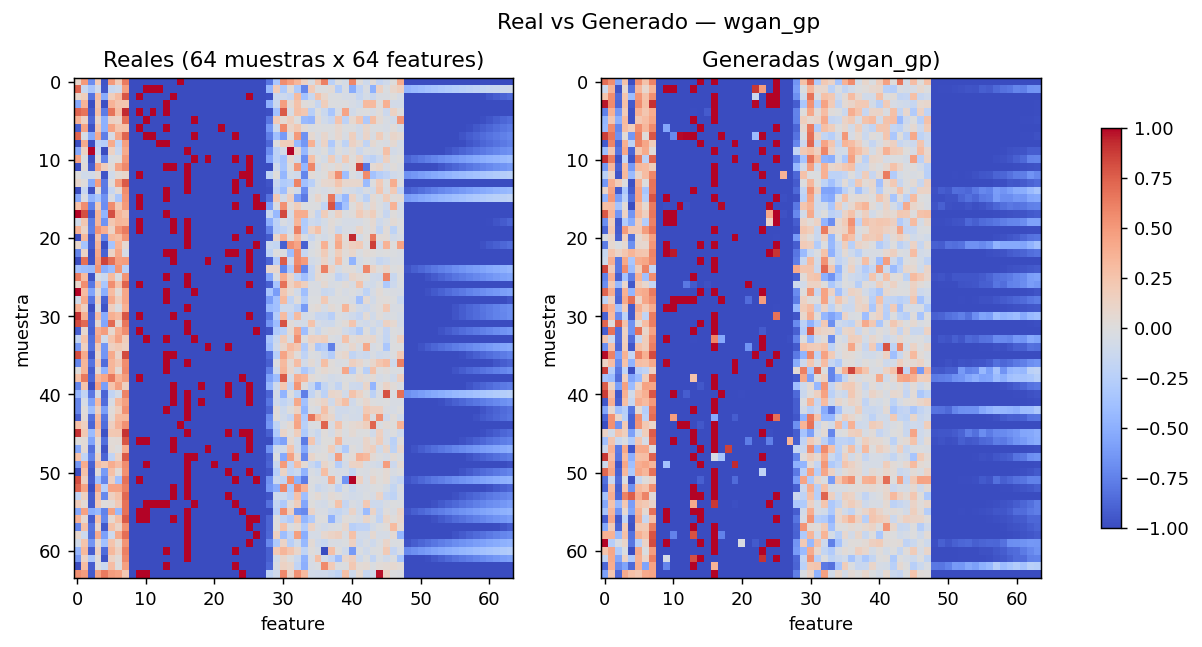
\includegraphics[width=\columnwidth]{figures/grid_real_vs_wgan_gp.png}
\caption{Real versus WGAN-GP generated profiles ($8\times8 = 64$ samples, 64 features each).
The generated block structure matches the real one. A similar figure for the Vanilla GAN is in
\texttt{runs/workshop5/grid\_real\_vs\_vanilla.png}. Source:
\texttt{runs/workshop5/grid\_real\_vs\_wgan\_gp.png}.}
\label{fig:grids}
\end{figure}

\begin{figure}[t]
\centering
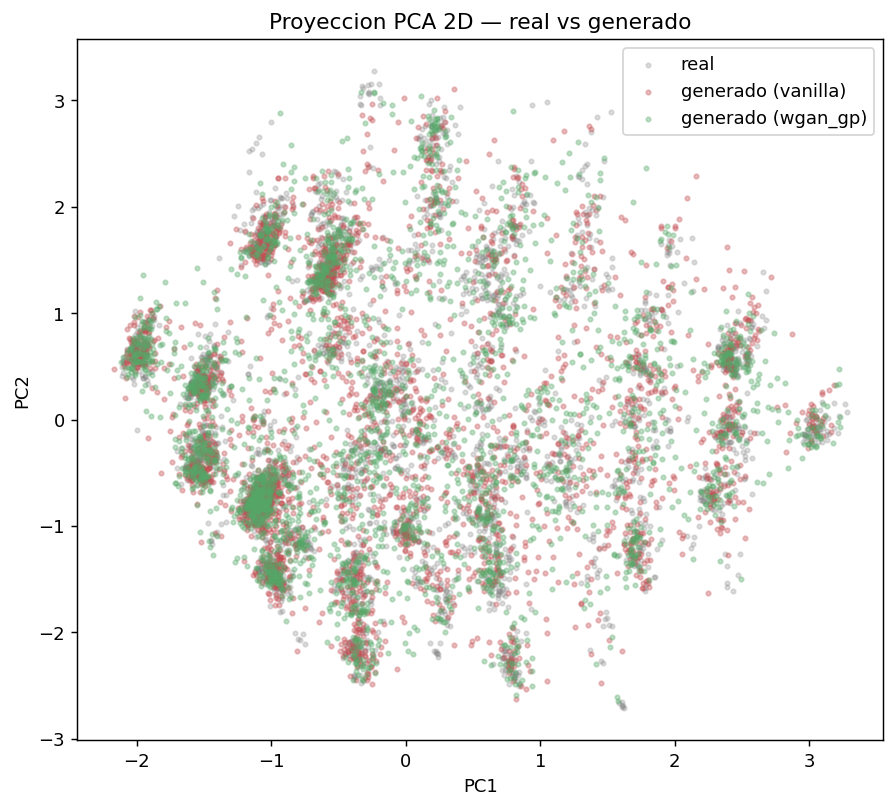
\includegraphics[width=\columnwidth]{figures/pca_real_vs_generated.png}
\caption{2D PCA projection of real (gray), Vanilla GAN (red), and WGAN-GP (green) samples. The
clouds overlap, which indicates good coverage and no mode collapse. Source:
\texttt{runs/workshop5/pca\_real\_vs\_generated.png}.}
\label{fig:pca}
\end{figure}

\begin{figure}[t]
\centering
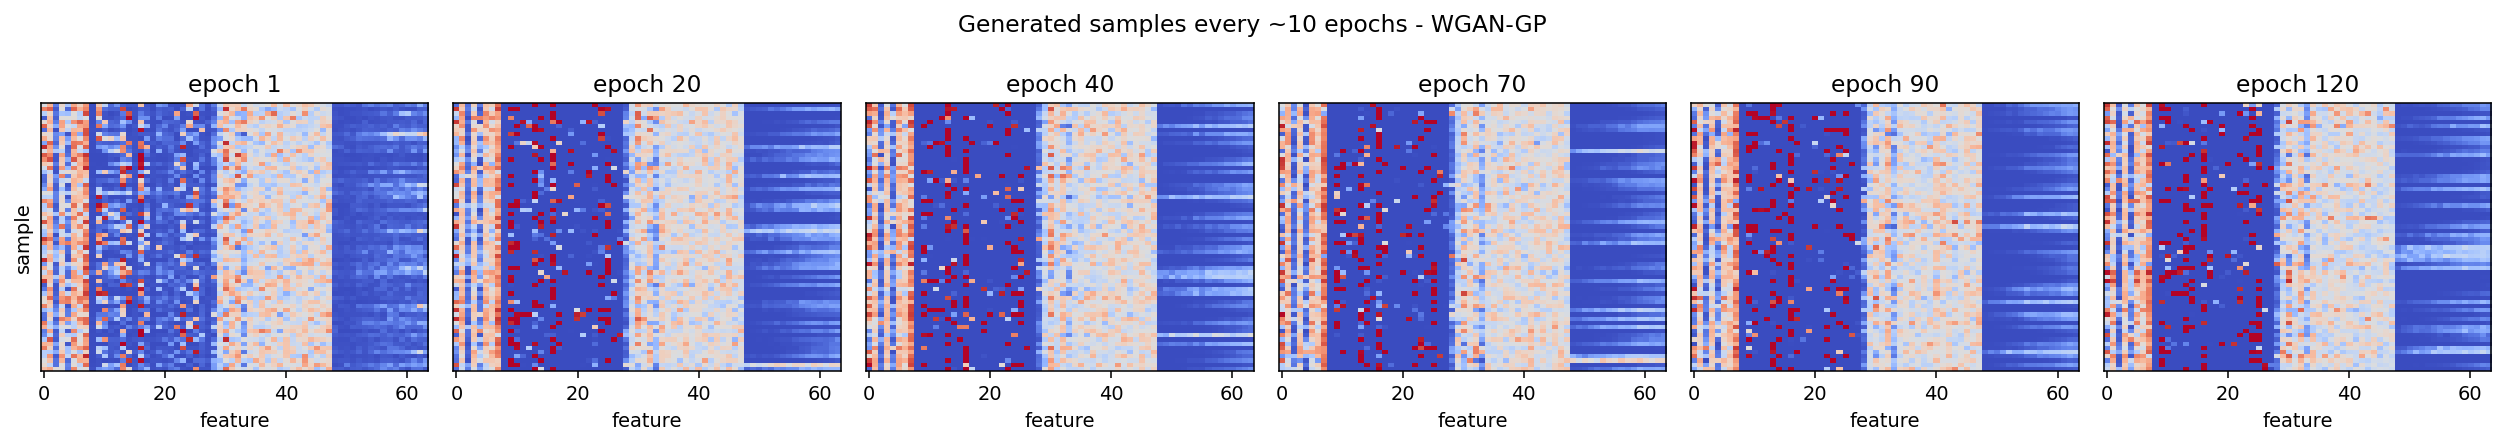
\includegraphics[width=\columnwidth]{figures/samples_grid_wgan.png}
\caption{WGAN-GP samples saved every 10 epochs, showing how the generator output becomes more
structured during training. Source: \texttt{runs/workshop5/samples\_grid\_wgan.png}.}
\label{fig:evolution}
\end{figure}

\subsection{Failure Mode Analysis}

The workshop asks us to document training pathologies. In our experiments the main risk was the
discriminator becoming too strong in the Vanilla GAN, which would make the generator gradient
vanish. We can see in Figure~\ref{fig:curves} that this did not happen in a severe way: the
discriminator accuracy on real samples even goes down to about $0.36$ in the middle of training,
so the discriminator did not dominate. The mitigation we used for this is one-sided label
smoothing (real labels $=0.9$) and dropout in the discriminator, and this was enough to keep a
balance. We did not observe mode collapse in either model, as the diversity ratios in
Table~\ref{tab:quality} are close to $1$ and the PCA clouds in Figure~\ref{fig:pca} cover the
real distribution. The only clear difference is quality: the Vanilla GAN produces noisier
samples than the WGAN-GP, which is a quality gap and not a collapse. Overall, the WGAN-GP was
both more stable (Wasserstein distance curve) and better in quality (Fr\'echet distance), which
matches the theory.

\subsection{Data Augmentation Experiment}

Table~\ref{tab:augment} reports the downstream \texttt{like} classifier under the four
conditions, evaluated on the held-out test split. The baseline with real data only reaches
F1~$=0.6650$ and ROC-AUC~$=0.8046$. Adding synthetic data changes the result only by a very
small margin: the Vanilla GAN gives $+0.0012$ in F1, the WGAN-GP gives $+0.0028$ in F1 (the best
case), and the cGAN gives $+0.0007$ in F1. The changes in ROC-AUC are also tiny and can be
positive or negative. In practice, these differences are inside the noise of the experiment, so
we cannot say that augmentation clearly improves the downstream model.

\begin{table}[t]
\centering
\caption{Data augmentation experiment. Downstream \texttt{like} classifier on the test split
under four conditions. $\Delta$F1 is the change against the real-only baseline. Source:
\texttt{runs/workshop5/augmentation\_results.json}.}
\label{tab:augment}
\small
\begin{tabular}{lccccc}
\toprule
Condition & Acc. & Prec. & Rec. & F1 & $\Delta$F1 \\
\midrule
(a) Real only        & 0.7382 & 0.6230 & 0.7131 & 0.6650 & --- \\
(b) + Vanilla        & 0.7390 & 0.6239 & 0.7148 & 0.6662 & +0.0012 \\
(c) + WGAN-GP        & 0.7339 & 0.6125 & 0.7341 & \textbf{0.6678} & +0.0028 \\
(d) + cGAN (bal.)    & 0.7411 & 0.6286 & 0.7075 & 0.6657 & +0.0007 \\
\bottomrule
\end{tabular}
\end{table}

\subsection{Cumulative Comparison Across Workshops}

Table~\ref{tab:cumulative} adds the Workshop 5 results to the cumulative comparison on the
binary \texttt{like} task. The numbers for Workshops 1, 2, and 4 are taken from the reports of
those workshops. We note that the Workshop 5 tabular classifier reaches the highest ROC-AUC in
the table ($0.8046$), slightly above the Workshop 2 \texttt{HybridNeuMF} ($0.7942$). This makes
sense, because the 64-D vectors already contain rich features derived from Workshops 1, 2, and
4, so the classifier starts from a very informative representation. The Workshop 4 VAE keeps the
highest F1 and recall, because it works as a one-class detector. Workshop 3 (reinforcement
learning) is not in this table, because it uses a different sequential protocol (episode return,
NDCG@K over sessions) that is not comparable with binary classification; we report it separately
in the Workshop 3 paper.

\begin{table*}[t]
\centering
\caption{Cumulative comparison across workshops on the binary \texttt{like} task (test set).
Workshops 1, 2, and 4 values are taken from the corresponding team reports. Workshop 3 (RL) uses
a sequential protocol and is reported separately. Source:
\texttt{runs/workshop5/cumulative\_comparison.csv}.}
\label{tab:cumulative}
\small
\begin{tabular}{llccccc}
\toprule
WS & Model & Acc. & Prec. & Rec. & F1 & ROC-AUC \\
\midrule
W1 & Random Forest Clf            & 0.7031 & 0.5773 & 0.6914 & 0.6293 & 0.7645 \\
W1 & Logistic Regression          & 0.7134 & 0.6026 & 0.6270 & 0.6146 & 0.7604 \\
W2 & HybridNeuMF                  & 0.7156 & 0.5838 & 0.7651 & 0.6623 & 0.7942 \\
W4 & VAE ($\beta=4.0$, ELBO)      & 0.6528 & 0.6620 & \textbf{0.9270} & \textbf{0.7724} & 0.6964 \\
W5 & Classifier (real only)       & 0.7382 & 0.6230 & 0.7131 & 0.6650 & 0.8046 \\
W5 & Classifier + Vanilla         & 0.7390 & 0.6239 & 0.7148 & 0.6662 & 0.8048 \\
W5 & Classifier + WGAN-GP         & 0.7339 & 0.6125 & 0.7341 & 0.6678 & 0.8043 \\
W5 & Classifier + cGAN            & 0.7411 & 0.6286 & 0.7075 & 0.6657 & 0.8046 \\
\bottomrule
\end{tabular}
\end{table*}

%=====================================================================
\section{Discussion}

\subsection{Why Did Augmentation Help So Little?}

The most important result to interpret is the small effect of augmentation. We see two main
reasons for this. First, the downstream classifier already has a lot of real signal: the
training data of the previous workshops has millions of real interactions, and even the
validation split used by the classifier has $33{,}092$ real examples, so adding a few thousand
synthetic samples is a small fraction of the data. Second, the Vanilla GAN and the WGAN-GP learn
the majority class (\texttt{like}~$=1$), which is already well represented, so they do not add
much new information. The cGAN can generate the minority class, but it was trained on fewer
examples (the validation split only), and the real signal is already enough, so it does not
change the result much either.

This result is coherent with the data augmentation literature. GAN-based augmentation is most
useful when the real data is scarce, as in the medical imaging case of
Frid-Adar et al.~\cite{fridadar2018}. In our case the real data is abundant and of good quality,
so the synthetic data has little to add. The positive side is that augmentation did not hurt the
model either, which was a real risk mentioned in the workshop guidelines: the quality of our
synthetic data (especially from the WGAN-GP) was good enough that it did not degrade the
downstream performance.

\subsection{What Characteristics of the Synthetic Data Matter?}

The experiment also suggests which properties of the synthetic data matter most. The WGAN-GP,
which has the lowest Fr\'echet distance and the best correlation preservation, is also the
condition with the best (though small) F1 gain. This supports the intuition that higher-quality
synthetic data is more useful for augmentation, even if the gain is small here. The class
balance also matters: the cGAN was our attempt to add the minority class, and although it did
not improve F1 in this regime, it is the right direction if the real data were more unbalanced
or scarce.

\subsection{Limitations and Threats to Validity}

Our study has several limitations. First, the downstream model is a tabular classifier and not
the Workshop 2 \texttt{HybridNeuMF}, because \texttt{HybridNeuMF} needs user/item indices and
cannot take synthetic feature vectors. This is a reasonable choice and follows the Frid-Adar
pipeline, but it means our augmentation result is about a feature-based classifier and not about
the exact Workshop 2 model. Second, the cGAN was trained on the validation split, because that
is the only split that exposes both classes in the Workshop 4 representation; this gives the cGAN
less data than the unconditional models. Third, our quality metrics are domain-specific and not
the standard Inception Score, because the data is tabular; this is correct for our case but makes
the numbers less directly comparable with image GAN papers. Finally, the synthetic data lives in
the 64-D feature space, so it inherits any bias already present in those features, including the
popularity bias and the cold-start effects that we discussed in the previous workshops.

%=====================================================================
\section{Conclusions and Future Work}

In this work we studied Generative Adversarial Networks as a way to generate synthetic
user--movie interaction profiles for the MovieLens 32M dataset, and we tested whether this
synthetic data can improve a downstream task through augmentation. We reused the same leak-free
chronological split and the same 64-dimensional interaction profiles from Workshops 1, 2, and 4,
so the experiment stays consistent with our previous work and avoids data leakage by
construction.

We draw four main conclusions. First, both the Vanilla GAN and the WGAN-GP can generate
realistic tabular profiles, and neither shows mode collapse (diversity ratio $0.9379$ and
$0.9687$). Second, the WGAN-GP is clearly the better and more stable model: its Wasserstein
distance converges smoothly, and its tabular Fr\'echet distance ($0.1107$) is about $6.6$ times
lower than that of the Vanilla GAN ($0.7327$), with better correlation preservation. This
confirms the theory that the gradient penalty gives a more stable training. Third, the data
augmentation experiment shows only a marginal change in the downstream \texttt{like} classifier
(best case $+0.0028$ in F1 with WGAN-GP), which we interpret as a consequence of already having
abundant and good-quality real data. Augmentation did not help much, but it also did not hurt,
which means that the synthetic data was realistic enough to be safe. Fourth, in the cumulative
comparison the feature-based classifier reaches a competitive ROC-AUC ($0.8046$), in line with
the supervised and unsupervised models of the previous workshops.

For future work, we see three directions. First, we could test the augmentation in a
low-data regime (for example, using only a small sample of real users), where GAN-based
augmentation is expected to help more. Second, we could train the cGAN on a larger set with both
classes, so that the minority class is better modeled. Third, we could extend the generator to
produce not only the 64-D profiles but also valid user/item indices, which would allow a direct
augmentation of the Workshop 2 \texttt{HybridNeuMF} model and a more complete comparison.

%=====================================================================
\begin{thebibliography}{99}
\small

\bibitem{goodfellow2014}
I. Goodfellow, J. Pouget-Abadie, M. Mirza, B. Xu, D. Warde-Farley, S. Ozair, A. Courville, and
Y. Bengio, ``Generative adversarial nets,'' in \emph{Advances in Neural Information Processing
Systems (NeurIPS)}, 2014, pp. 2672--2680.

\bibitem{radford2015}
A. Radford, L. Metz, and S. Chintala, ``Unsupervised representation learning with deep
convolutional generative adversarial networks,'' in \emph{Proc. Int. Conf. Learn. Represent.
(ICLR)}, 2016.

\bibitem{arjovsky2017}
M. Arjovsky, S. Chintala, and L. Bottou, ``Wasserstein GAN,'' in \emph{Proc. 34th Int. Conf.
Machine Learning (ICML)}, 2017, pp. 214--223.

\bibitem{gulrajani2017}
I. Gulrajani, F. Ahmed, M. Arjovsky, V. Dumoulin, and A. Courville, ``Improved training of
Wasserstein GANs,'' in \emph{Advances in Neural Information Processing Systems (NeurIPS)}, 2017,
pp. 5767--5777.

\bibitem{fridadar2018}
M. Frid-Adar, I. Diamant, E. Klang, M. Amitai, J. Goldberger, and H. Greenspan, ``GAN-based
synthetic medical image augmentation for increased CNN performance in liver lesion
classification,'' \emph{Neurocomputing}, vol. 321, pp. 321--331, 2018.

\bibitem{salimans2016}
T. Salimans, I. Goodfellow, W. Zaremba, V. Cheung, A. Radford, and X. Chen, ``Improved
techniques for training GANs,'' in \emph{Advances in Neural Information Processing Systems
(NeurIPS)}, 2016, pp. 2234--2242.

\bibitem{heusel2017}
M. Heusel, H. Ramsauer, T. Unterthiner, B. Nessler, and S. Hochreiter, ``GANs trained by a two
time-scale update rule converge to a local Nash equilibrium,'' in \emph{Advances in Neural
Information Processing Systems (NeurIPS)}, 2017, pp. 6626--6637.

\bibitem{isola2016}
P. Isola, J.-Y. Zhu, T. Zhou, and A. A. Efros, ``Image-to-image translation with conditional
adversarial networks,'' in \emph{Proc. IEEE Conf. Computer Vision and Pattern Recognition
(CVPR)}, 2017, pp. 1125--1134.

\bibitem{harper2015}
F. M. Harper and J. A. Konstan, ``The MovieLens datasets: History and context,'' \emph{ACM
Trans. Interact. Intell. Syst. (TiiS)}, vol. 5, no. 4, pp. 1--19, 2015.

\bibitem{koren2009}
Y. Koren, R. Bell, and C. Volinsky, ``Matrix factorization techniques for recommender systems,''
\emph{Computer}, vol. 42, no. 8, pp. 30--37, 2009.

\bibitem{he2017}
X. He, L. Liao, H. Zhang, L. Nie, X. Hu, and T.-S. Chua, ``Neural collaborative filtering,'' in
\emph{Proc. 26th Int. Conf. World Wide Web (WWW)}, 2017, pp. 173--182.

\end{thebibliography}

\end{document}
